%%%%%%%%%%%%%%%%%%%%%%%%%%%%%%%%%%%%%%%%%%%%%%%%%%%%%%%%%%%%%%%%%%%%%%%%%%%%%%%%
%%%%%%%%%%%%%%%%%%%%%%%%%%%%%%%%%%%%%%%%%%%%%%%%%%%%%%%%%%%%%%%%%%%%%%%%%%%%%%%%
%%%%%%%%%%%%%%%%%%%%%%%%%%%%%%%%%%%%%%%%%%%%%%%%%%%%%%%%%%%%%%%%%%%%%%%%%%%%%%%%
%%%%%%%%%%%%%%%%%%%%%%%%%%%%%%%%%%%%%%%%%%%%%%%%%%%%%%%%%%%%%%%%%%%%%%%%%%%%%%%%
\chapter{Correction des systèmes asservis\label{chap-correc}}
%%%%%%%%%%%%%%%%%%%%%%%%%%%%%%%%%%%%%%%%%%%%%%%%%%%%%%%%%%%%%%%%%%%%%%%%%%%%%%%%
%%%%%%%%%%%%%%%%%%%%%%%%%%%%%%%%%%%%%%%%%%%%%%%%%%%%%%%%%%%%%%%%%%%%%%%%%%%%%%%%
%%%%%%%%%%%%%%%%%%%%%%%%%%%%%%%%%%%%%%%%%%%%%%%%%%%%%%%%%%%%%%%%%%%%%%%%%%%%%%%%
%%%%%%%%%%%%%%%%%%%%%%%%%%%%%%%%%%%%%%%%%%%%%%%%%%%%%%%%%%%%%%%%%%%%%%%%%%%%%%%%
\minitoc
\newpage
%%%%%%%%%%%%%%%%%%%%%%%%%%%%%%%%%%%%%%%%%%%%%%%%%%%%%%%%%%%%%%%%%%%%%%%%%%%%%%%%
%%%%%%%%%%%%%%%%%%%%%%%%%%%%%%%%%%%%%%%%%%%%%%%%%%%%%%%%%%%%%%%%%%%%%%%%%%%%%%%%
%%%%%%%%%%%%%%%%%%%%%%%%%%%%%%%%%%%%%%%%%%%%%%%%%%%%%%%%%%%%%%%%%%%%%%%%%%%%%%%%
\section{Nécessité de la correction}
%%%%%%%%%%%%%%%%%%%%%%%%%%%%%%%%%%%%%%%%%%%%%%%%%%%%%%%%%%%%%%%%%%%%%%%%%%%%%%%%
%%%%%%%%%%%%%%%%%%%%%%%%%%%%%%%%%%%%%%%%%%%%%%%%%%%%%%%%%%%%%%%%%%%%%%%%%%%%%%%%
%%%%%%%%%%%%%%%%%%%%%%%%%%%%%%%%%%%%%%%%%%%%%%%%%%%%%%%%%%%%%%%%%%%%%%%%%%%%%%%%

%%%%%%%%%%%%%%%%%%%%%%%%%%%%%%%%%%%%%%%%%%%%%%%%%%%%%%%%%%%%%%%%%%%%%%%%%%%%%%%%
%%%%%%%%%%%%%%%%%%%%%%%%%%%%%%%%%%%%%%%%%%%%%%%%%%%%%%%%%%%%%%%%%%%%%%%%%%%%%%%%
%%%%%%%%%%%%%%%%%%%%%%%%%%%%%%%%%%%%%%%%%%%%%%%%%%%%%%%%%%%%%%%%%%%%%%%%%%%%%%%%
\section{Structure de la correction}
%%%%%%%%%%%%%%%%%%%%%%%%%%%%%%%%%%%%%%%%%%%%%%%%%%%%%%%%%%%%%%%%%%%%%%%%%%%%%%%%
%%%%%%%%%%%%%%%%%%%%%%%%%%%%%%%%%%%%%%%%%%%%%%%%%%%%%%%%%%%%%%%%%%%%%%%%%%%%%%%%
%%%%%%%%%%%%%%%%%%%%%%%%%%%%%%%%%%%%%%%%%%%%%%%%%%%%%%%%%%%%%%%%%%%%%%%%%%%%%%%%
\textbf{La correction élabore une commande $u(t)$ à partir d'un écart 
$\epsilon(t)$}


\begin{center}
    \tikzsetnextfilename{bs_correction_chap_correction-ext}
    \begin{tikzpicture}
    \bs[$\epsilon(p)$][$C(p)$][Correcteur][$U(p)$]
\end{tikzpicture}

\end{center}


%%%%%%%%%%%%%%%%%%%%%%%%%%%%%%%%%%%%%%%%%%%%%%%%%%%%%%%%%%%%%%%%%%%%%%%%%%%%%%%%
%%%%%%%%%%%%%%%%%%%%%%%%%%%%%%%%%%%%%%%%%%%%%%%%%%%%%%%%%%%%%%%%%%%%%%%%%%%%%%%%
%%%%%%%%%%%%%%%%%%%%%%%%%%%%%%%%%%%%%%%%%%%%%%%%%%%%%%%%%%%%%%%%%%%%%%%%%%%%%%%%
\section{Correcteur P, I et D}
%%%%%%%%%%%%%%%%%%%%%%%%%%%%%%%%%%%%%%%%%%%%%%%%%%%%%%%%%%%%%%%%%%%%%%%%%%%%%%%%
%%%%%%%%%%%%%%%%%%%%%%%%%%%%%%%%%%%%%%%%%%%%%%%%%%%%%%%%%%%%%%%%%%%%%%%%%%%%%%%%
%%%%%%%%%%%%%%%%%%%%%%%%%%%%%%%%%%%%%%%%%%%%%%%%%%%%%%%%%%%%%%%%%%%%%%%%%%%%%%%%
\index{Correcteur ! Proportionnel (P)}
\index{Correcteur ! Intégral (I)}
\index{Correcteur ! Dérivé (D)}
%%%%%%%%%%%%%%%%%%%%%%%%%%%%%%%%%%%%%%%%%%%%%%%%%%%%%%%%%%%%%%%%%%%%%%%%%%%%%%%%
%%%%%%%%%%%%%%%%%%%%%%%%%%%%%%%%%%%%%%%%%%%%%%%%%%%%%%%%%%%%%%%%%%%%%%%%%%%%%%%%
%%%%%%%%%%%%%%%%%%%%%%%%%%%%%%%%%%%%%%%%%%%%%%%%%%%%%%%%%%%%%%%%%%%%%%%%%%%%%%%%
\section{Correcteur PI et PD}
%%%%%%%%%%%%%%%%%%%%%%%%%%%%%%%%%%%%%%%%%%%%%%%%%%%%%%%%%%%%%%%%%%%%%%%%%%%%%%%%
%%%%%%%%%%%%%%%%%%%%%%%%%%%%%%%%%%%%%%%%%%%%%%%%%%%%%%%%%%%%%%%%%%%%%%%%%%%%%%%%
%%%%%%%%%%%%%%%%%%%%%%%%%%%%%%%%%%%%%%%%%%%%%%%%%%%%%%%%%%%%%%%%%%%%%%%%%%%%%%%%

\index{Correcteur ! Proportionnel Intégral (PI)}
\index{Correcteur ! Proportionnel Dérivé (PD)}

%%%%%%%%%%%%%%%%%%%%%%%%%%%%%%%%%%%%%%%%%%%%%%%%%%%%%%%%%%%%%%%%%%%%%%%%%%%%%%%%
%%%%%%%%%%%%%%%%%%%%%%%%%%%%%%%%%%%%%%%%%%%%%%%%%%%%%%%%%%%%%%%%%%%%%%%%%%%%%%%%
%%%%%%%%%%%%%%%%%%%%%%%%%%%%%%%%%%%%%%%%%%%%%%%%%%%%%%%%%%%%%%%%%%%%%%%%%%%%%%%%
\section{Correcteur à avance et retard de phase}
%%%%%%%%%%%%%%%%%%%%%%%%%%%%%%%%%%%%%%%%%%%%%%%%%%%%%%%%%%%%%%%%%%%%%%%%%%%%%%%%
%%%%%%%%%%%%%%%%%%%%%%%%%%%%%%%%%%%%%%%%%%%%%%%%%%%%%%%%%%%%%%%%%%%%%%%%%%%%%%%%
%%%%%%%%%%%%%%%%%%%%%%%%%%%%%%%%%%%%%%%%%%%%%%%%%%%%%%%%%%%%%%%%%%%%%%%%%%%%%%%%
\index{Correcteur ! à avance de phase (AP)}

Le correcteur à avance de phase (AP) est défini par la fonction de transfert :
\[
    C_{AP}(p)=\dfrac{1+\alpha\tau p}{1+\tau p} 
\]
avec $\alpha>1$.

\begin{center}
    \tikzsetnextfilename{bode_avancedephase_chap_correction-ext}
    \begin{tikzpicture}[trim axis left]
    \begin{axis}[
    ticklabel style = {font=\footnotesize},
    width=0.9\textwidth,
    height=0.25\textheight,
    ylabel={Gain (\si{\decibel})},
    xtick={1e-4,1e-3,1e-2,1e-1,1,1e1,1e2,1e3,1e4,1e5},
    ytick={0,1,2,3,4,5,6,7,8,9,10,11,12,13,14,15},
    xticklabels={$10^{-4}$,$10^{-3}$,$10^{-2}$,$10^{-1}$,
                 $10^{0}$,$10^{1}$,$10^{2}$,$10^{3}$,$10^{4}$,$10^{5}$},
    yticklabels={0,,2,,4,,6,,8,,10,,12,,14},
    xmode=log,ymode=normal,
    xmin=1e-2, xmax=1e2,
    ymin=0, ymax=15,
    grid=both,
    major grid style={black!40},
    clip=false,
]
    \pgfmathsetmacro{\aa}{5.0} 
    \pgfmathsetmacro{\ia}{(1/\aa)} 
    \pgfmathsetmacro{\wm}{(1/sqrt(\aa))} 
    \pgfmathsetmacro{\gm}{10*log10(\aa)} 
    \pgfmathsetmacro{\dgm}{20*log10(\aa)} 
    \addplot[ultra thick, col1,domain=1e-2:1e2, samples=201]    
            {10*log10(1+\aa*\aa*x*x)-10*log10(1+x*x)};
    \addplot[line width=2pt,col4,dashed,domain=1e0:1e2, samples=51] 
            {20*log10(\aa)};
    \addplot[line width=2pt,col4,dashed,domain=1e-2:\ia, samples=51] {0};
    \addplot[line width=2pt,col4,dashed,domain=\ia:1e0, samples=101] 
            {20*log10(\aa)+20*log10(x)};
    \draw[line width=2pt,col2,-latex] 
         (axis cs:\wm,0) node[below] {$\omega_m$}  -- 
         node[right] {$\boldsymbol{10\log{\alpha}}$} (axis cs:\wm,\gm);
    \draw[line width=2pt,col2,-latex] 
        (axis cs:10,0)  --
        node[right] {$\boldsymbol{20\log{\alpha}}$} (axis cs:10,\dgm);
\end{axis}
\end{tikzpicture}

\begin{tikzpicture}[trim axis left]
\begin{axis}[
    ticklabel style = {font=\footnotesize},
    width=0.9\textwidth,
    height=0.25\textheight,
    xlabel={Pulsation (\si{\radian\per\second})},
    ylabel={Phase (\degree)},
    xtick={1e-4,1e-3,1e-2,1e-1,1,1e1,1e2,1e3,1e4,1e5},
    ytick={0,15,30,45,60,75,90},
    yticklabels={0,,30,,60,,90},
    xticklabels={$10^{-4}$,$10^{-3}$,$10^{-2}$,$10^{-1}$,$10^{0}$,
                 $10^{1}$,$10^{2}$,$10^{3}$,$10^{4}$,$10^{5}$},
    xmode=log,ymode=normal,
    xmin=1e-2, xmax=1e2,
    ymin=0, ymax=90,
    grid=both,
    major grid style={black!40},
    clip=false
]
    \pgfmathsetmacro{\aa}{5.0} 
    \pgfmathsetmacro{\ia}{(1/\aa)} 
    \pgfmathsetmacro{\wm}{(1/sqrt(\aa))} 
    \pgfmathsetmacro{\pm}{atan((\aa-1)/(2*sqrt(\aa)))} 
    \addplot[ultra thick, col1,domain=1e-2:1e2, samples=201] 
    {atan2(\aa*x,1)-atan2(x,1)};
    \addplot[line width=2pt,col4,dashed,domain=1e-2:\ia, samples=51] {0};
    \addplot[line width=2pt,col4,dashed,domain=\ia:1e0, samples=51] {90};
    \addplot[line width=2pt,col4,dashed,domain=1e0:1e2, samples=51] {0};
    \draw[line width=2pt,col4,dashed] 
    (axis cs:1e0,0)  -- (axis cs:1e0,90);
    \draw[line width=2pt,col4,dashed] 
    (axis cs:\ia,90)  -- (axis cs:\ia,0);
    \draw[line width=2pt,col2,-latex] 
    (axis cs:\wm,0)   node[below] {$\omega_m$}  -- 
    (axis cs:\wm,\pm) node[xshift=-1,above] 
    {\tiny$\boldsymbol{\arctan{\left(\dfrac{\alpha-1}
                                           {2\sqrt{\alpha}}\right)}}$};
\end{axis}
\end{tikzpicture}

\end{center}

Le maximum de la phase se trouve à la moyenne géométrique du segment 
$\left[\dfrac{1}{\alpha\tau},\dfrac{1}{\alpha}\right]$ (l'echelle étant logarithmique 
ceux sont les rapports qui sont égaux)
\[
    \omega_m^2=\dfrac{1}{\alpha\tau^2}
\]
ou encore 
\[
    \omega_m=\dfrac{1}{\sqrt{\alpha}\tau}
\]
Pour $\alpha=5$ et $\tau=1$ on a alors $\omega_m=\SI{1}{\sqrt{5}}\sim\SI{0.44}{\radian\per\second}$.
\[
    \phi(\omega)=\arg{(C_{AP}(\jw))}=\arctan{\alpha\tau\omega_m}-\arctan{\tau\omega_m}
\]

\[
    \phi_m=\phi(\omega_m)=\arctan{\alpha\tau\omega_m}-\arctan{\tau\omega_m}
\]
en utilisant la relation trigonométrique pour $\tan{(a-b)}$ et en posant $a=\arctan{\alpha\tau\omega_m}$ 
et $b=\arctan{\tau\omega_m}$, on écrit:
\[
    \tan{\phi(\omega_m)}=\dfrac{\alpha\tau\omega_m-\tau\omega_m}{1+\alpha\tau^2\omega_m^2}
                        =\dfrac{\alpha-1}{2\sqrt{\alpha}}
\]
donc on a :
\[
    \phi_m=\arctan{\left(\dfrac{\alpha-1}{2\sqrt{\alpha}}\right)}
\]
Une autre forme possible est également donnée par (en notant que $\sin\arctan{x}=\dfrac{x}{\sqrt{1+x^2}}$):
\[
    \phi_m=\arcsin{\left(\dfrac{\alpha-1}{\alpha+1}\right)}
\]
On remarquera que le maximum ne dépend pas de $\tau$.
Pour $\alpha=5$, $\phi_m=\SI{41.8}{\degree}$.

Le gain pour la pulsation $\omega_m$ est donné par:
\[
    C_{AP,\si{\dB}}(j\omega_m)=10\log{(1+\alpha^2\tau^2\omega_m^2)}-
                               10\log{(1+\tau^2\omega_m^2)}
\]
puisque $\tau^2\omega_m^2=\dfrac{1}{\alpha}$.
\[
    C_{AP,\si{\dB}}(j\omega_m)=10\log{1+\alpha}-10\log{\dfrac{1+\alpha}{\alpha}}=10\log{\alpha}
\]

%%%%%%%%%%%%%%%%%%%%%%%%%%%%%%%%%%%%%%%%%%%%%%%%%%%%%%%%%%%%%%%%%%%%%%%%%%%%%%%%
%%%%%%%%%%%%%%%%%%%%%%%%%%%%%%%%%%%%%%%%%%%%%%%%%%%%%%%%%%%%%%%%%%%%%%%%%%%%%%%%
\subsection{Correcteur à retard de phase}
%%%%%%%%%%%%%%%%%%%%%%%%%%%%%%%%%%%%%%%%%%%%%%%%%%%%%%%%%%%%%%%%%%%%%%%%%%%%%%%%
%%%%%%%%%%%%%%%%%%%%%%%%%%%%%%%%%%%%%%%%%%%%%%%%%%%%%%%%%%%%%%%%%%%%%%%%%%%%%%%%
\index{Correcteur ! à retard de phase (RP)}
Le correcteur à retard de phase (RP) est défini par la fonction de transfert :
\[
    C_{RP}(p)=\dfrac{1+\tau p}{1+\beta\tau p}
\]
avec $\beta>1$

\begin{center}
    \tikzsetnextfilename{bode_retarddephase_chap_correction-ext}
    \begin{tikzpicture}[trim axis left]
\begin{axis}[
    ticklabel style = {font=\footnotesize},
    width=0.9\textwidth,
    height=0.25\textheight,
    ylabel={Gain (\si{\decibel})},
    xtick={1e-4,1e-3,1e-2,1e-1,1,1e1,1e2,1e3,1e4,1e5},
    ytick={-15,-14,-13,-12,-11,-10,-9,-8,-7,-6,-5,-4,-3,-2,-1,0},
    xticklabels={$10^{-4}$,$10^{-3}$,$10^{-2}$,$10^{-1}$,$10^{0}$,$10^{1}$,$10^{2}$,$10^{3}$,$10^{4}$,$10^{5}$},
    yticklabels={,-14,,-12,,-10,,-8,,-6,,-4,,-2,,0},
    xmode=log,ymode=normal,
    xmin=1e-2, xmax=1e2,
    ymin=-15, ymax=0,
    grid=both,
    major grid style={black!40},
    clip=false,
]
    \pgfmathsetmacro{\bb}{5.0} 
    \pgfmathsetmacro{\ib}{(1/\bb)} 
    \pgfmathsetmacro{\wm}{(1/sqrt(\bb))} 
    \pgfmathsetmacro{\gm}{10*log10(\bb)} 
    \pgfmathsetmacro{\dgm}{20*log10(\bb)} 
    \addplot[ultra thick, col1,domain=1e-2:1e2, samples=201]   {10*log10(1+x*x)-10*log10(1+\bb*\bb*x*x)};
    \addplot[line width=2pt,col4,dashed,domain=1e-2:\ib, samples=51] {0};
    \addplot[line width=2pt,col4,dashed,domain=\ib:1e0, samples=101] {-20*log10(\bb)-20*log10(x)};
    \addplot[line width=2pt,col4,dashed,domain=1e0:1e2, samples=51] {-20*log10(\bb)};
    \draw[line width=2pt,col2,-latex] (axis cs:\wm,0) node[above] {$\omega_m$}  -- 
                                      node[right] {$\boldsymbol{10\log{\alpha}}$} (axis cs:\wm,-\gm);
    \draw[line width=2pt,col2,-latex] (axis cs:10,0)  -- node[right] {$\boldsymbol{20\log{\alpha}}$} 
                                      (axis cs:10,-\dgm);
\end{axis}
\end{tikzpicture}

\begin{tikzpicture}[trim axis left]
\begin{axis}[
    ticklabel style = {font=\footnotesize},
    width=0.9\textwidth,
    height=0.25\textheight,
    xlabel={Pulsation (\si{\radian\per\second})},
    ylabel={Phase (\degree)},
    xtick={1e-4,1e-3,1e-2,1e-1,1,1e1,1e2,1e3,1e4,1e5},
    ytick={-90,-75,-60,-45,-30,-15,0},
    yticklabels={-90,,-60,,-30,,0},
    xticklabels={$10^{-4}$,$10^{-3}$,$10^{-2}$,$10^{-1}$,$10^{0}$,$10^{1}$,$10^{2}$,$10^{3}$,$10^{4}$,$10^{5}$},
    xmode=log,ymode=normal,
    xmin=1e-2, xmax=1e2,
    ymin=-90, ymax=0,
    grid=both,
    major grid style={black!40},
    clip=false
]
    \pgfmathsetmacro{\bb}{5.0} 
    \pgfmathsetmacro{\ib}{(1/\bb)} 
    \pgfmathsetmacro{\wm}{(1/sqrt(\bb))} 
    \pgfmathsetmacro{\pm}{-atan((\bb-1)/(2*sqrt(\bb)))} 
    \addplot[ultra thick,col1,domain=1e-2:1e2,samples=201] {atan2(x,1)-atan2(\bb*x,1)};
    \addplot[line width=2pt,col4,dashed,domain=1e-2:\ib, samples=51] {0};
    \addplot[line width=2pt,col4,dashed,domain=\ib:1e0, samples=51] {-90};
    \addplot[line width=2pt,col4,dashed,domain=1e0:1e2, samples=51] {0};
    \draw[line width=2pt,col4,dashed] (axis cs:1e0,0)    -- (axis cs:1e0,-90);
    \draw[line width=2pt,col4,dashed] (axis cs:\ib,-90)  -- (axis cs:\ib,0);
    \draw[line width=2pt,col2,-latex] (axis cs:\wm,0) node[above] {$\omega_m$}  
                                   -- (axis cs:\wm,\pm) node[xshift=-1,below] 
                                      {\tiny$\boldsymbol{\arctan{\left(\dfrac{\alpha-1}{2\sqrt{\alpha}}\right)}}$};
\end{axis}
\end{tikzpicture}

\end{center}

Le minimum de la phase se trouve à la moyenne géométrique du segment 
$\left[\dfrac{1}{\beta\tau},\dfrac{1}{\tau}\right]$. Cette pulsation 
est donnée par :
\[
    \omega_m=\dfrac{1}{\sqrt{\beta}\tau}
\]

Pour $\beta=5$ et $\tau=1$ on a alors $\omega_m=\SI{1}{\sqrt{5}}\sim\SI{0.44}{\radian\per\second}$.
\[
    \phi(\omega)=\arg{(C_{RP}(\jw))}=\arctan{\tau\omega_m}-\arctan{\beta\tau\omega_m}
\]

\[
    \phi_m=\phi(\omega_m)=\arctan{\tau\omega_m}-\arctan{\beta\tau\omega_m}
\]
en utilisant la relation trigonométrique pour $\tan{(a-b)}$ et en posant $a=\arctan{\tau\omega_m}$ 
et $b=\arctan{\beta\tau\omega_m}$, on écrit:
\[
    \tan{\phi(\omega_m)}=\dfrac{\tau\omega_m-\beta\tau\omega_m}{1+\beta\tau^2\omega_m^2}
                        =\dfrac{1-\beta}{2\sqrt{\beta}}
\]
donc on a :
\[
    \phi_m=\arctan{\left(\dfrac{1-\beta}{2\sqrt{\beta}}\right)}
\]
On remarquera que le maximum ne dépend pas de $\tau$.
Pour $\beta=5$, $\phi_m=\SI{-41.8}{\degree}$.

Le gain pour la pulsation $\omega_m$ est donné par:
\[
    C_{RP,\si{\dB}}(j\omega_m)=10\log{(1+\tau^2\omega_m^2)}-
                               10\log{(1+\beta^2\tau^2\omega_m^2)}
\]
puisque $\tau^2\omega_m^2=\dfrac{1}{\beta}$.
\[
    C_{RP,\si{\dB}}(j\omega_m)=10\log{\left(\dfrac{1+\beta}{\beta}\right)}-10\log{\left(1+\beta\right)}=-10\log{\beta}
\]

%%%%%%%%%%%%%%%%%%%%%%%%%%%%%%%%%%%%%%%%%%%%%%%%%%%%%%%%%%%%%%%%%%%%%%%%%%%%%%%%
%%%%%%%%%%%%%%%%%%%%%%%%%%%%%%%%%%%%%%%%%%%%%%%%%%%%%%%%%%%%%%%%%%%%%%%%%%%%%%%%
\subsection{Correcteur à retard-avance de phase}
%%%%%%%%%%%%%%%%%%%%%%%%%%%%%%%%%%%%%%%%%%%%%%%%%%%%%%%%%%%%%%%%%%%%%%%%%%%%%%%%
%%%%%%%%%%%%%%%%%%%%%%%%%%%%%%%%%%%%%%%%%%%%%%%%%%%%%%%%%%%%%%%%%%%%%%%%%%%%%%%%
\index{Correcteur ! à retard-avance de phase}
Le correcteur à retard-avance de phase (RAP) est défini par la fonction de transfert :
\[
    C_{RAP}(p)=\dfrac{1+\tau_r p}{1+\beta\tau_r p}\cdot\dfrac{1+\alpha\tau_a p}{1+\tau_a p}
\]
avec $\alpha>1$ et $\beta>1$. On prendra $\alpha=\beta$.

\begin{center}
    \tikzsetnextfilename{bode_retardavancedephase_chap_correction-ext}
    \begin{tikzpicture}[trim axis left]
\begin{axis}[
    ticklabel style = {font=\footnotesize},
    width=0.9\textwidth,
    height=0.25\textheight,
    ylabel={Gain (\si{\decibel})},
    xtick={1e-4,1e-3,1e-2,1e-1,1,1e1,1e2,1e3,1e4,1e5},
    ytick={-20,-18,-16,-14,-12,-10,-8,-6,-4,-2,0},
    xticklabels={$10^{-4}$,$10^{-3}$,$10^{-2}$,$10^{-1}$,$10^{0}$,$10^{1}$,$10^{2}$,$10^{3}$,$10^{4}$,$10^{5}$},
    yticklabels={-20,,-16,,-12,,-8,,-4,,0},
    xmode=log,ymode=normal,
    xmin=1e-2, xmax=1e3,
    ymin=-20, ymax=0,
    grid=both,
    major grid style={black!40},
    clip=false,
]
    \pgfmathsetmacro{\ta}{0.02} 
    \pgfmathsetmacro{\tb}{0.25} 
    \pgfmathsetmacro{\aa}{5} 
    \pgfmathsetmacro{\bb}{5} 
    \pgfmathsetmacro{\ib}{(1/(\bb*\tb))} 
    \pgfmathsetmacro{\ia}{(1/(\aa*\ta))} 
    \pgfmathsetmacro{\itb}{(1/\tb)} 
    \pgfmathsetmacro{\ita}{(1/\ta)} 
    \pgfmathsetmacro{\wm}{(1/sqrt(\bb))} 
    \pgfmathsetmacro{\gm}{10*log10(\bb)} 
    \pgfmathsetmacro{\dgm}{20*log10(\bb)} 
    \addplot[ultra thick, col1,domain=1e-2:1e3, samples=201]   {10*log10(1+\tb*\tb*x*x)+
                                                                10*log10(1+\aa*\aa*\ta*\ta*x*x)-        
                                                                10*log10(1+\tb*\tb*\bb*\bb*x*x)-
                                                                10*log10(1+\ta*\ta*x*x)};
    \addplot[line width=2pt,col4,dashed,domain=1e-2:\ib, samples=51] {0};
    \addplot[line width=2pt,col4,dashed,domain=\ib:\itb, samples=101] {-20*log10(\bb*\tb)-20*log10(x)};
    \addplot[line width=2pt,col4,dashed,domain=\itb:\ia, samples=51] {-20*log10(\bb)};
    \addplot[line width=2pt,col4,dashed,domain=\ia:\ita, samples=51] {20*log10(\ta)+20*log10(x)};
    \addplot[line width=2pt,col4,dashed,domain=\ita:1e3, samples=51] {0};
\end{axis}
\end{tikzpicture}

\begin{tikzpicture}[trim axis left]
\begin{axis}[
    ticklabel style = {font=\footnotesize},
    width=0.9\textwidth,
    height=0.25\textheight,
    xlabel={Pulsation (\si{\radian\per\second})},
    ylabel={Phase (\degree)},
    xtick={1e-4,1e-3,1e-2,1e-1,1,1e1,1e2,1e3,1e4,1e5},
    ytick={-90,-75,-60,-45,-30,-15,0,15,30,45,60,75,90},
    yticklabels={-90,,-60,,-30,,0,,30,,60,,90},
    xticklabels={$10^{-4}$,$10^{-3}$,$10^{-2}$,$10^{-1}$,$10^{0}$,$10^{1}$,$10^{2}$,$10^{3}$,$10^{4}$,$10^{5}$},
    xmode=log,ymode=normal,
    xmin=1e-2, xmax=1e3,
    ymin=-90, ymax=90,
    grid=both,
    major grid style={black!40},
    clip=false
]
    \pgfmathsetmacro{\ta}{0.02} 
    \pgfmathsetmacro{\tb}{0.25} 
    \pgfmathsetmacro{\aa}{5} 
    \pgfmathsetmacro{\bb}{5} 
    \pgfmathsetmacro{\ib}{(1/(\bb*\tb))} 
    \pgfmathsetmacro{\ia}{(1/(\aa*\ta))} 
    \pgfmathsetmacro{\itb}{(1/\tb)} 
    \pgfmathsetmacro{\ita}{(1/\ta)} 
    \pgfmathsetmacro{\wm}{(1/sqrt(\bb))} 
    \pgfmathsetmacro{\pm}{-atan((\bb-1)/(2*sqrt(\bb)))} 
    \addplot[ultra thick,col1,domain=1e-2:1e3,samples=201] {atan2(\aa*\ta*x,1)+atan2(\tb*x,1)-atan2(\tb*\bb*x,1)-atan2(\ta*x,1)};
    \addplot[line width=2pt,col4,dashed,domain=1e-2:\ib, samples=51] {0};
    \addplot[line width=2pt,col4,dashed,domain=\ib:\itb, samples=51] {-90};
    \addplot[line width=2pt,col4,dashed,domain=\itb:\ia, samples=51] {0};
    \addplot[line width=2pt,col4,dashed,domain=\ia:\ita, samples=51] {90};
    \addplot[line width=2pt,col4,dashed,domain=\ita:1e3, samples=51] {0};
    \draw[line width=2pt,col4,dashed] (axis cs:\ib,0)    -- (axis cs:\ib,-90);
    \draw[line width=2pt,col4,dashed] (axis cs:\itb,-90)    -- (axis cs:\itb,0);
    \draw[line width=2pt,col4,dashed] (axis cs:\ia,0)    -- (axis cs:\ia,90);
    \draw[line width=2pt,col4,dashed] (axis cs:\ita,90)    -- (axis cs:\ita,0);
\end{axis}
\end{tikzpicture}

\end{center}
%%%%%%%%%%%%%%%%%%%%%%%%%%%%%%%%%%%%%%%%%%%%%%%%%%%%%%%%%%%%%%%%%%%%%%%%%%%%%%%%
%%%%%%%%%%%%%%%%%%%%%%%%%%%%%%%%%%%%%%%%%%%%%%%%%%%%%%%%%%%%%%%%%%%%%%%%%%%%%%%%
%%%%%%%%%%%%%%%%%%%%%%%%%%%%%%%%%%%%%%%%%%%%%%%%%%%%%%%%%%%%%%%%%%%%%%%%%%%%%%%%
\section{Correcteur PID}
%%%%%%%%%%%%%%%%%%%%%%%%%%%%%%%%%%%%%%%%%%%%%%%%%%%%%%%%%%%%%%%%%%%%%%%%%%%%%%%%
%%%%%%%%%%%%%%%%%%%%%%%%%%%%%%%%%%%%%%%%%%%%%%%%%%%%%%%%%%%%%%%%%%%%%%%%%%%%%%%%
%%%%%%%%%%%%%%%%%%%%%%%%%%%%%%%%%%%%%%%%%%%%%%%%%%%%%%%%%%%%%%%%%%%%%%%%%%%%%%%%
\index{Correcteur ! Proportionnele Intégral Dérivé (PID)}
%\newpage
%%%%%%%%%%%%%%%%%%%%%%%%%%%%%%%%%%%%%%%%%%%%%%%%%%%%%%%%%%%%%%%%%%%%%%%%%%%%%%%%
%%%%%%%%%%%%%%%%%%%%%%%%%%%%%%%%%%%%%%%%%%%%%%%%%%%%%%%%%%%%%%%%%%%%%%%%%%%%%%%%
%%%%%%%%%%%%%%%%%%%%%%%%%%%%%%%%%%%%%%%%%%%%%%%%%%%%%%%%%%%%%%%%%%%%%%%%%%%%%%%%
\section{Exercices du chapitre}
%%%%%%%%%%%%%%%%%%%%%%%%%%%%%%%%%%%%%%%%%%%%%%%%%%%%%%%%%%%%%%%%%%%%%%%%%%%%%%%%
%%%%%%%%%%%%%%%%%%%%%%%%%%%%%%%%%%%%%%%%%%%%%%%%%%%%%%%%%%%%%%%%%%%%%%%%%%%%%%%%
%%%%%%%%%%%%%%%%%%%%%%%%%%%%%%%%%%%%%%%%%%%%%%%%%%%%%%%%%%%%%%%%%%%%%%%%%%%%%%%%
%\newpage
%%%%%%%%%%%%%%%%%%%%%%%%%%%%%%%%%%%%%%%%%%%%%%%%%%%%%%%%%%%%%%%%%%%%%%%%%%%%%%%%
%%%%%%%%%%%%%%%%%%%%%%%%%%%%%%%%%%%%%%%%%%%%%%%%%%%%%%%%%%%%%%%%%%%%%%%%%%%%%%%%
%%%%%%%%%%%%%%%%%%%%%%%%%%%%%%%%%%%%%%%%%%%%%%%%%%%%%%%%%%%%%%%%%%%%%%%%%%%%%%%%
\section{Corrigé des exercices}
%%%%%%%%%%%%%%%%%%%%%%%%%%%%%%%%%%%%%%%%%%%%%%%%%%%%%%%%%%%%%%%%%%%%%%%%%%%%%%%%
%%%%%%%%%%%%%%%%%%%%%%%%%%%%%%%%%%%%%%%%%%%%%%%%%%%%%%%%%%%%%%%%%%%%%%%%%%%%%%%%
%%%%%%%%%%%%%%%%%%%%%%%%%%%%%%%%%%%%%%%%%%%%%%%%%%%%%%%%%%%%%%%%%%%%%%%%%%%%%%%%


%%%%%%%%%%%%%%%%%%%%%%%%%%%%%%%%%%%%%%%%%%%%%%%%%%%%%%%%%%%%%%%%%%%%%%%%%%%%%%%%
%%%%%%%%%%%%%%%%%%%%%%%%%%%%%%%%%%%%%%%%%%%%%%%%%%%%%%%%%%%%%%%%%%%%%%%%%%%%%%%%
%%%%%%%%%%%%%%%%%%%%%%%%%%%%%%%%%%%%%%%%%%%%%%%%%%%%%%%%%%%%%%%%%%%%%%%%%%%%%%%%
%%%%%%%%%%%%%%%%%%%%%%%%%%%%%%%%%%%%%%%%%%%%%%%%%%%%%%%%%%%%%%%%%%%%%%%%%%%%%%%%
%chap_correction.tex
